
\section{Numerical results \label{sec:num}}
\subsection{Accuracy}
In this section, we demonstrate the accuracy of the proposed numerical method (both in the {\it weak} sense 
described above, 
as well as in the classical sense after sufficiently many re-solves) on the triangular domain shown below. 
The reference solution for each of the examples is computed using a discretization with
a graded mesh in the vicinity of the corners, where the smallest panel at the corner is $2^{-200}$ times
the length of the first macroscopic panel away from the corner (see~\cref{fig:dom}). In these examples, the solutions are computed via dense linear solves.

\begin{figure}
\begin{center}
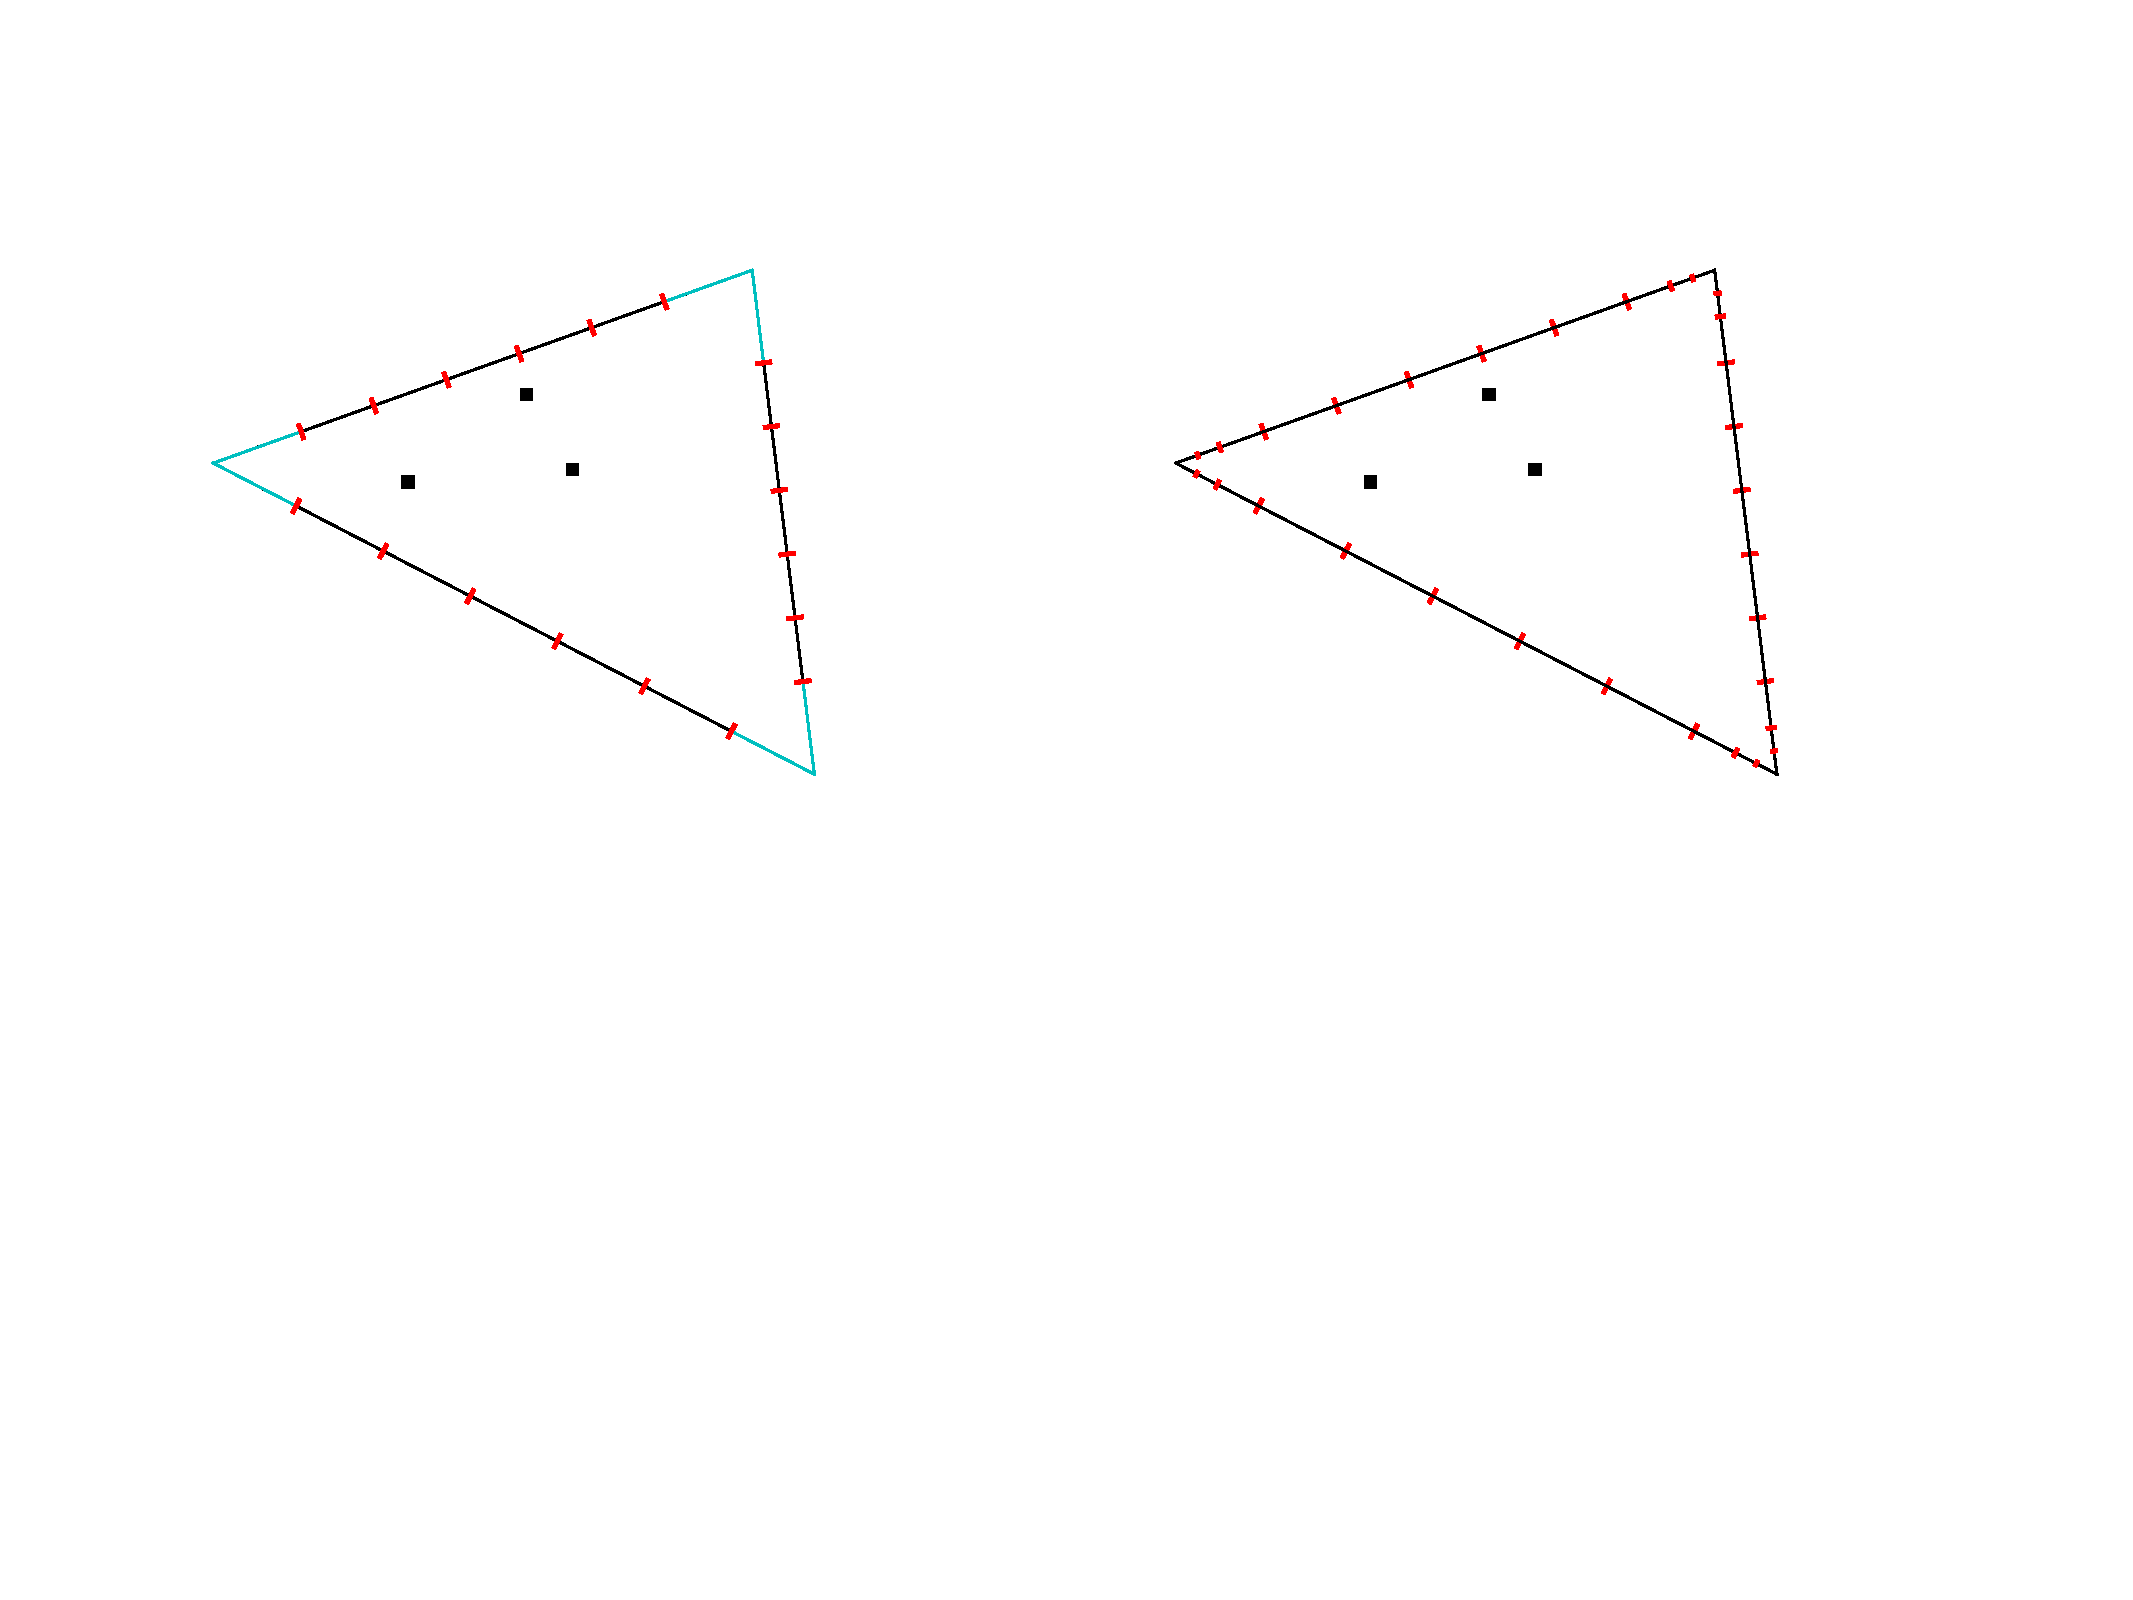
\includegraphics[width=0.7\linewidth]{paper-figs/discretization}
\caption{Problem domain and panel discretization of the boundary. The discretization on the left is based on using the Dirichlet
discretization at corner panels (indicated by blue panels) discussed in~\cref{sec:disc_dir}, while the discretization on the right is a sample discretization with 2 levels of refinement in the vicinity of the corner. All the panels in black are discretized using scaled Gauss-Legendre nodes. The square ticks indicate location of the charges $\bx_{j}$ for defining the boundary data for the scattering problem.}
\label{fig:dom}
\end{center}
\end{figure}

\begin{rem}
Though $2^{-200}$ is significantly smaller than machine precision, the matrix entries corresponding to the
corner interactions can be computed accurately by translating the corners to the origin when 
computing interactions of nearby points.
\end{rem} 
\begin{rem}
Simple arguments from complex analysis show that when using graded meshes, in order to obtain full 
machine precision 
($\sim 1.11 \times 10^{-16}$) for solutions of the Neumann problem at any point in the interior 
at least $10^{-16}$ away from a corner, it suffices to choose the smallest panel (i.e. the size of the 
panel closest to the corner) to be of size $2^{-100}.$ However, resulting values of the density will not be 
accurate to machine precision at all nodes. In fact the quality
of the density deteriorates as one approaches the corner. Thus, in order to obtain accurate point values
of the density to machine precision at all points which are at least $2^{-100}$ away from the corner, we use a smallest
panel size of $2^{-200}$. 
\end{rem}


The potential at target locations which are sufficiently far from the boundary (i.e. at least one panel length away from 
every panel) is the inner product of the 
density with a smooth function and hence can be computed accurately without re-solving (see~\cref{rem:far-field-accuracy}). For a target 
location $\boldsymbol{y}$, we compute the potential via the formula,
\begin{equation}
\label{eq:farfieldpot}
u(\by) = \int_{\Gamma} G(\bx,\by) \sigma(\bx) dS_{\bx} \approx \sum_{i=1}^{N}  G(\gamma(s_{i}),\by) \sigma_{i} \sqrt{w_{i}}
\end{equation}
In~\cref{fig:scatteringtest}, we compute the error in the solution at target
locations for a scattering problem whose right hand side is given by a collection of three interior charges
\begin{equation}
\label{eq:scatboundarydata}
f(\bx) = -\nabla  \left(\sum_{j=1}^{3} \log |\bx - \bx_{j}|  \right)  \cdot \bnu(\bx)\, ,  
\end{equation}
where the locations $\bx_{j}$ are denoted by square dots in~\cref{fig:scatteringtest}. Note that the density $\sigma$ plotted
as a function of arclength goes to infinity at the corner vertices, indicating that the native Dirichlet discretization 
presented in~\cref{sec:disc_dir} wouldn't have sufficed. However, the potential in the volume is accurate to 14 digits at
target locations away from the boundary. 
\begin{figure}
\begin{center}
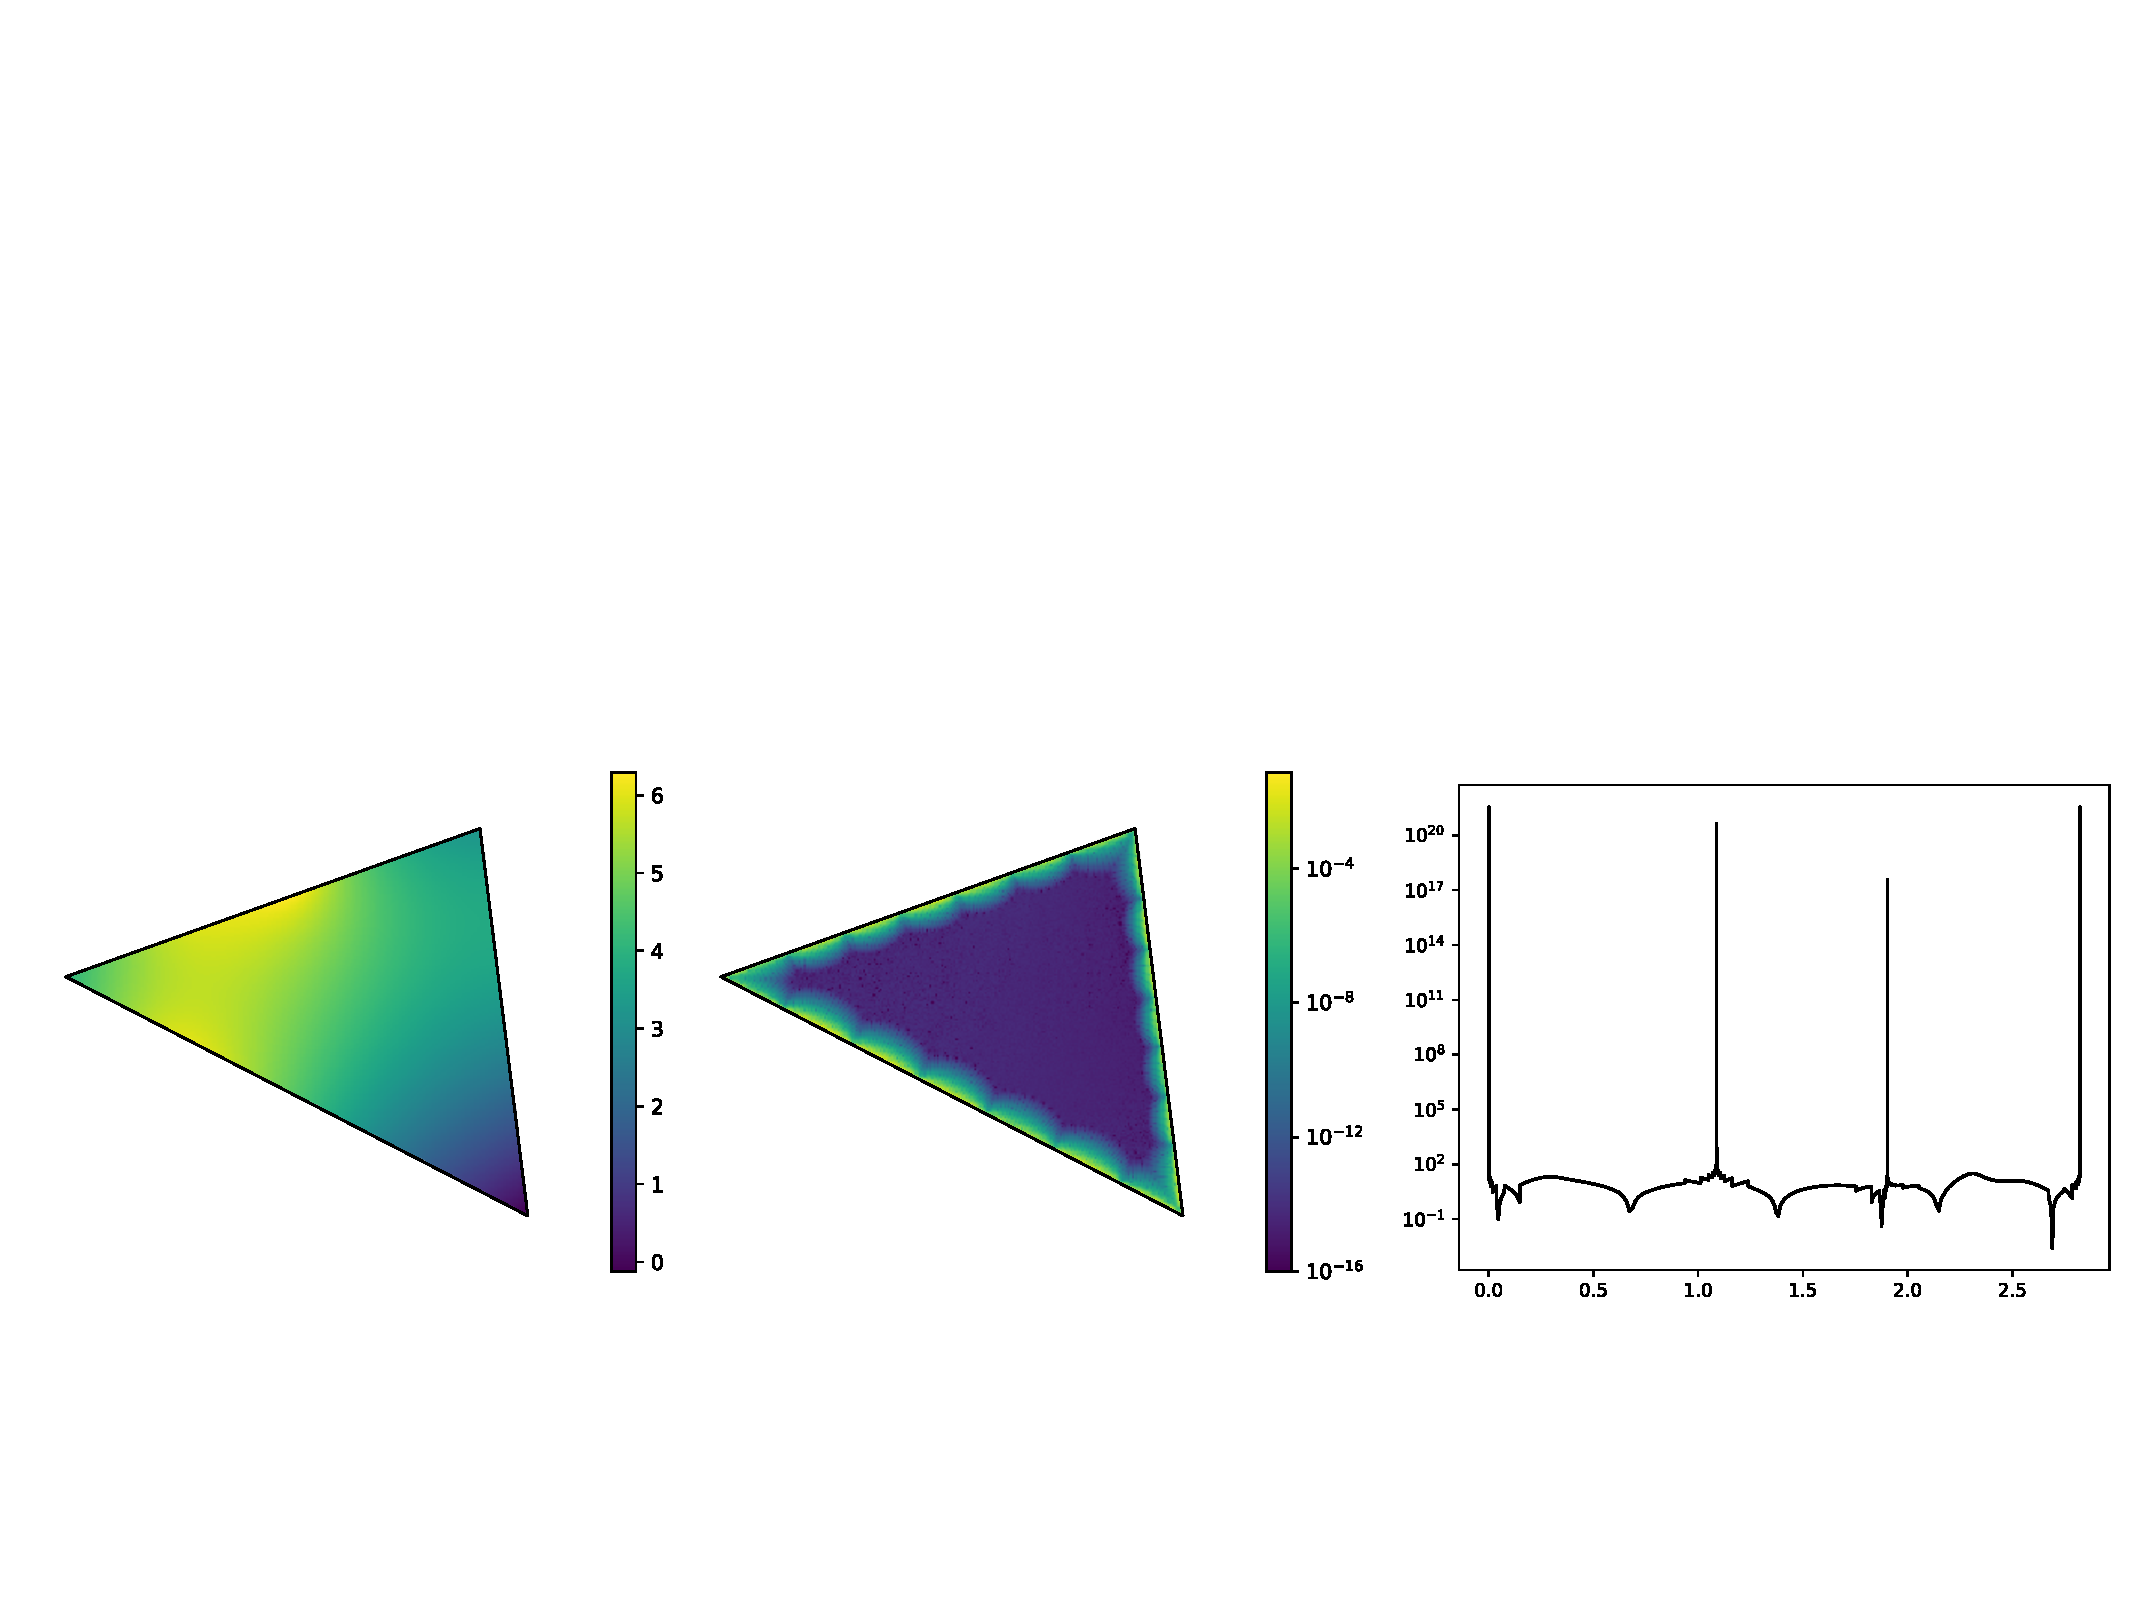
\includegraphics[width=\linewidth]{paper-figs/weaktest}
\caption{Left panel: Solution to Neumann problem with data given by~\cref{eq:scatboundarydata}, center panel: error in computing the potential in the formula using the underlying smooth quadrature~\cref{eq:farfieldpot}, and on the right the density $\sigma$ as a function of arc-length}.
\label{fig:scatteringtest}
\end{center}
\end{figure}


Another example of a ``weak quantity'' is the polarization tensor associated with a domain. This requires the solution of the
exterior problems with boundary data $f_{1} = \bnu_{1}$ or $f_{2} = \bnu_{2}$. Let $\sigma_{1}$ and $\sigma_{2}$ denote
the corresponding solutions. The polarization tensor can be expressed in terms of the solutions $\sigma_{1}$ and $\sigma_{2}$
as
\begin{equation}
P = \begin{bmatrix}
\int_{\Gamma} x_{1} \sigma_{1}(\bx) dS_{\bx} & \int_{\Gamma} x_{2} \sigma_{1}(\bx) dS_{\bx} \\
\int_{\Gamma} x_{1} \sigma_{2}(\bx) dS_{\bx} & \int_{\Gamma} x_{2} \sigma_{2}(\bx) dS_{\bx} 
\end{bmatrix}
\end{equation}
The polarization tensor as computed by the reference solution, and the error in computation using the adjoint discretization
are given by
\begin{equation}
P = \begin{bmatrix}
-0.823641009939200 & -0.139714174784448 \\
 -0.139714174784448 &  -1.1421444446470226
\end{bmatrix} \, , \quad \text{Error} = 
\begin{bmatrix} 
2.3 \times 10^{-15} & 7.9 \times 10^{-16} \\
1.3 \times. 10^{-14} & 2.7 \times 10^{-15}
\end{bmatrix}
\end{equation}

In order to demonstrate the accuracy of the corner re-solving approach in obtaining the true density at the corner panels, we  apply the procedure
discussed in~\cref{sec:resolve} iteratively, and compare the obtained density with the reference density after 20,40,60, and
80 iterations of resolves in the vicinity of one of the corners. The reference density and the errors are shown in ~\cref{fig:dens-error}. Furthermore, to highlight the need for special purpose discretizations in the vicinity of corners in the adjoint discretization, we also compare the solution computed using a graded mesh in the vicinity of corners, where the size of the smallest panels for both discretizations are equal. 

\begin{figure}
\begin{center}
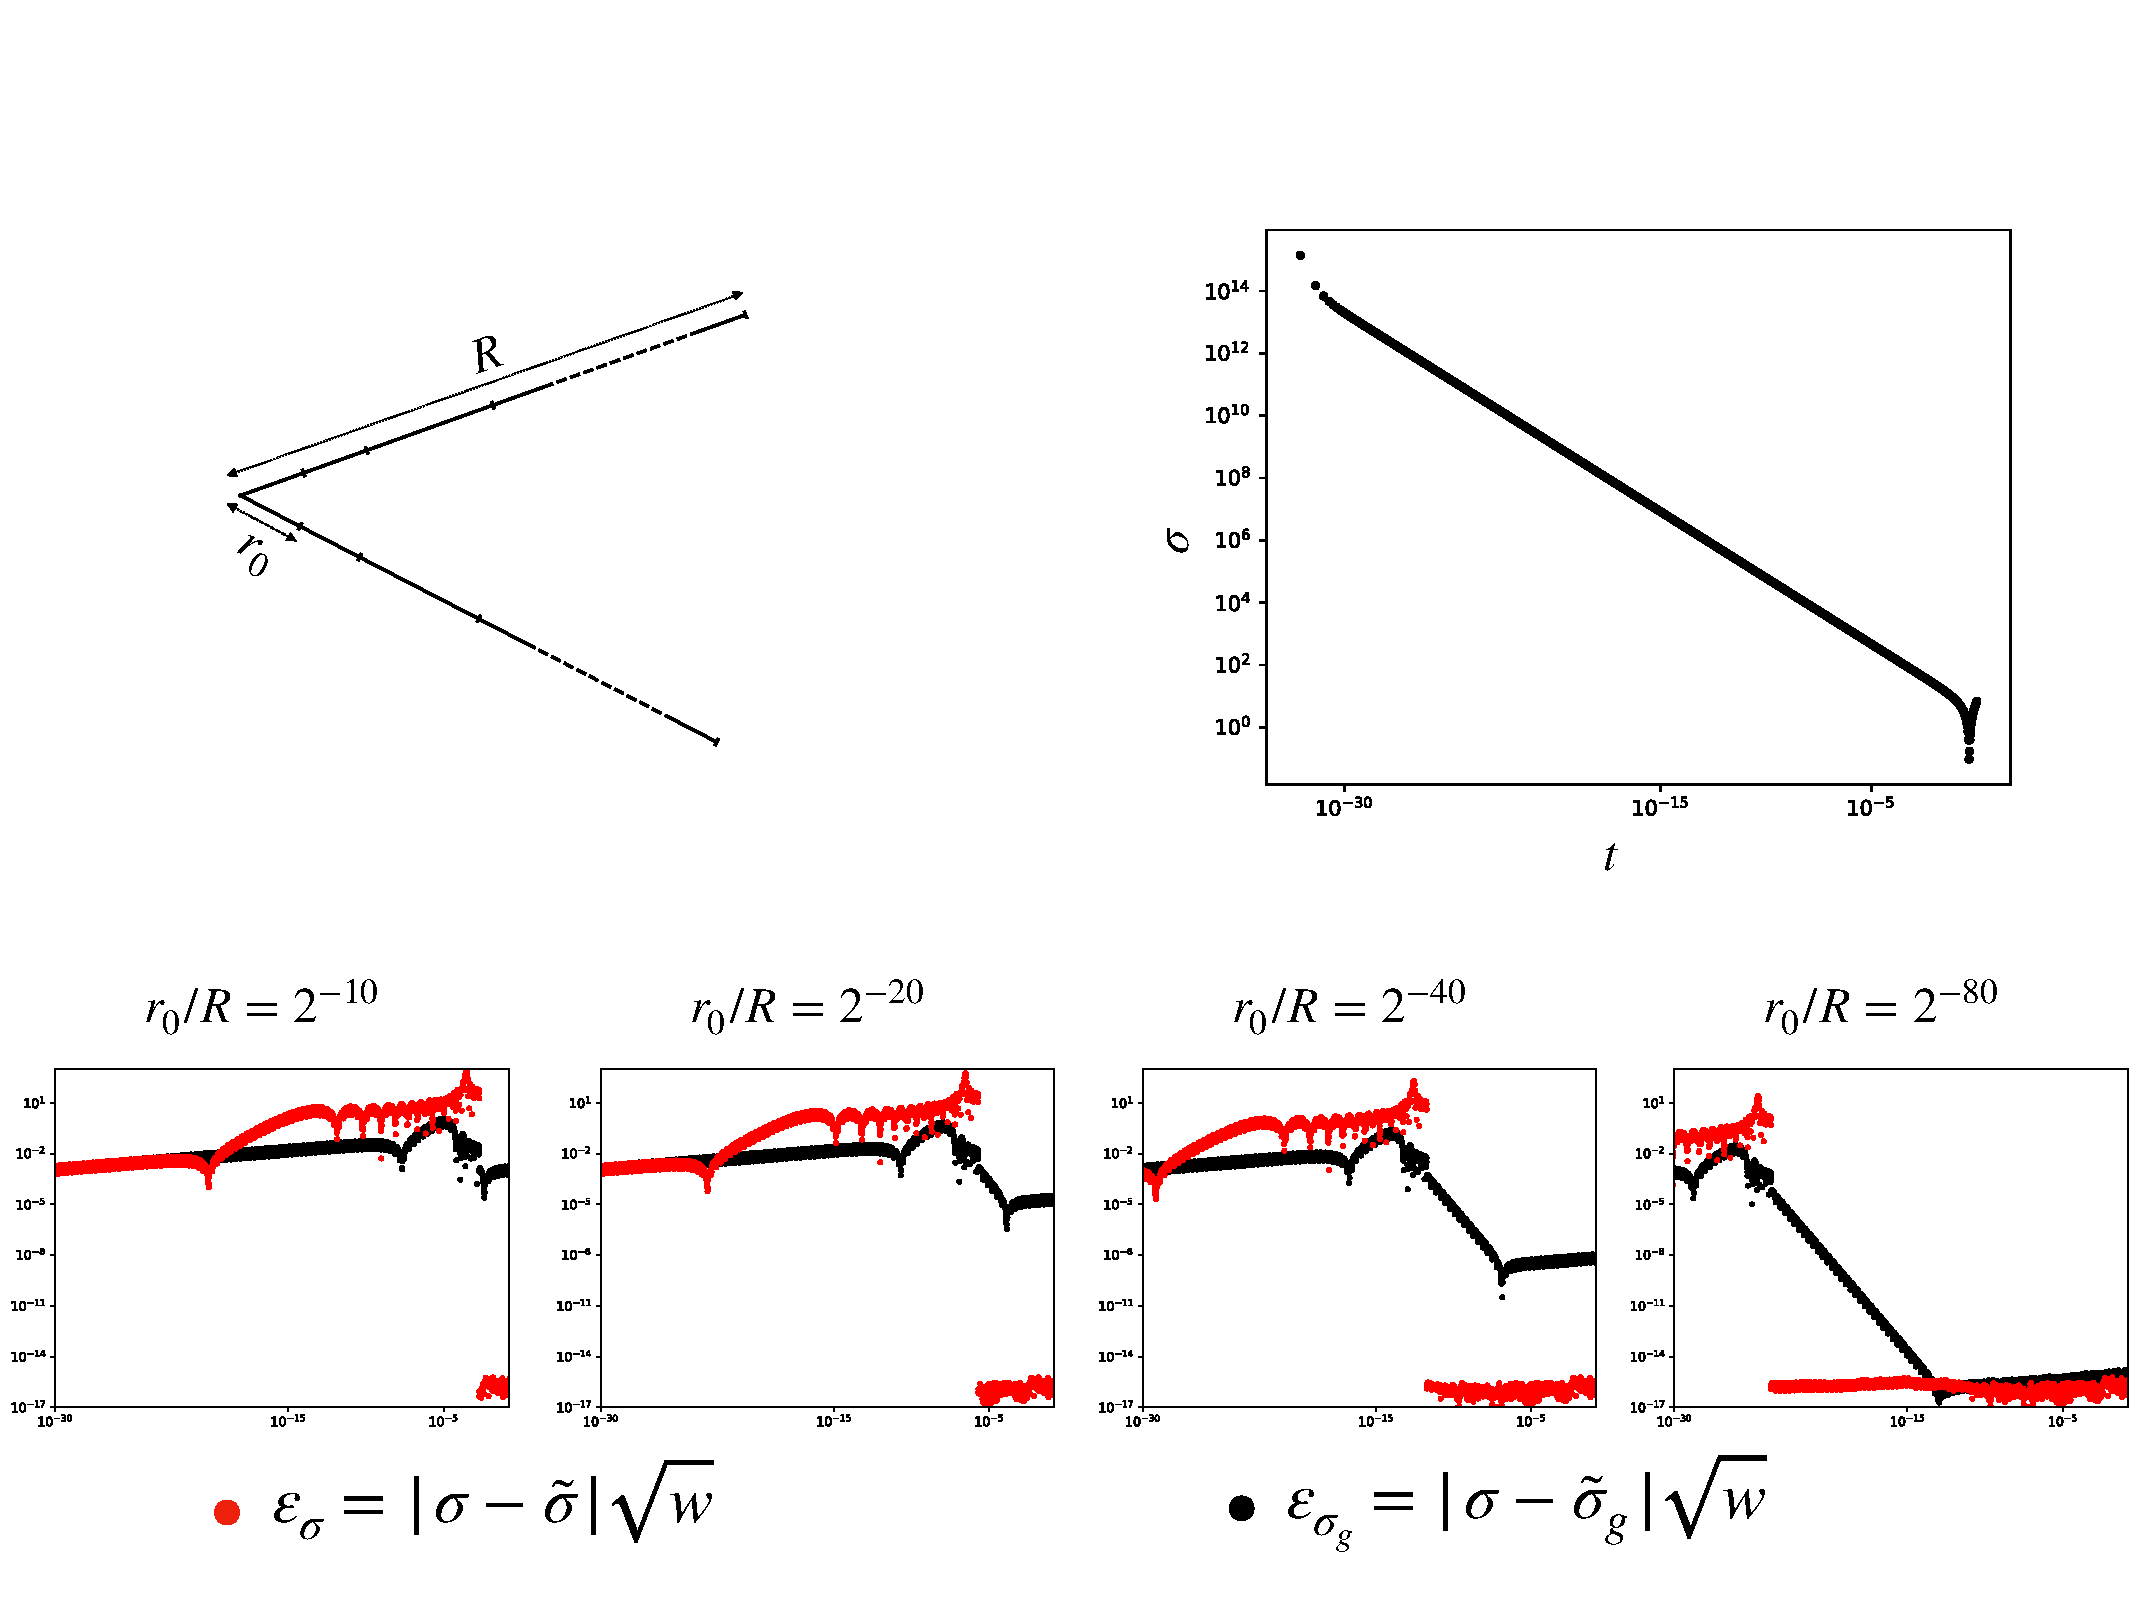
\includegraphics[width=\linewidth]{paper-figs/density}
\caption{Top row: (left) Illustrative mesh used for iteratively computing the solution in the vicinity of a corner, (right) the density in the vicinity of one of the corner panels. Bottom row: error in computing the density, where $\tilde{\sigma}$ denotes the density computed using special purpose discretizations at corner panels, and $\tilde{\sigma_{g}}$ denotes the density using a graded mesh with the smallest panel equal to the length of the smallest panel after the iterative resolve procedure. The errors are scaled by square roots of the quadrature weights.    }.
\label{fig:dens-error}
\end{center}
\end{figure}

After re-solving the density, the solution is evaluated on a tensor product polar grid, where the grid
is exponentially spaced in the radial direction and equispaced in the angular direction. For evaluation points (targets)
close to panels which are not at the corner, we use adaptive integration in order to resolve the near-singular behavior of
the kernel for accurate computation of the integrals. For target locations close to the corner panel, since we do not have
the capability to interpolate the density, we use the underlying smooth quadrature rules for computing their contribution. 
The reference solution and the errors are demonstrated in~\cref{fig:vol-plot}.
\begin{figure}
\begin{center}
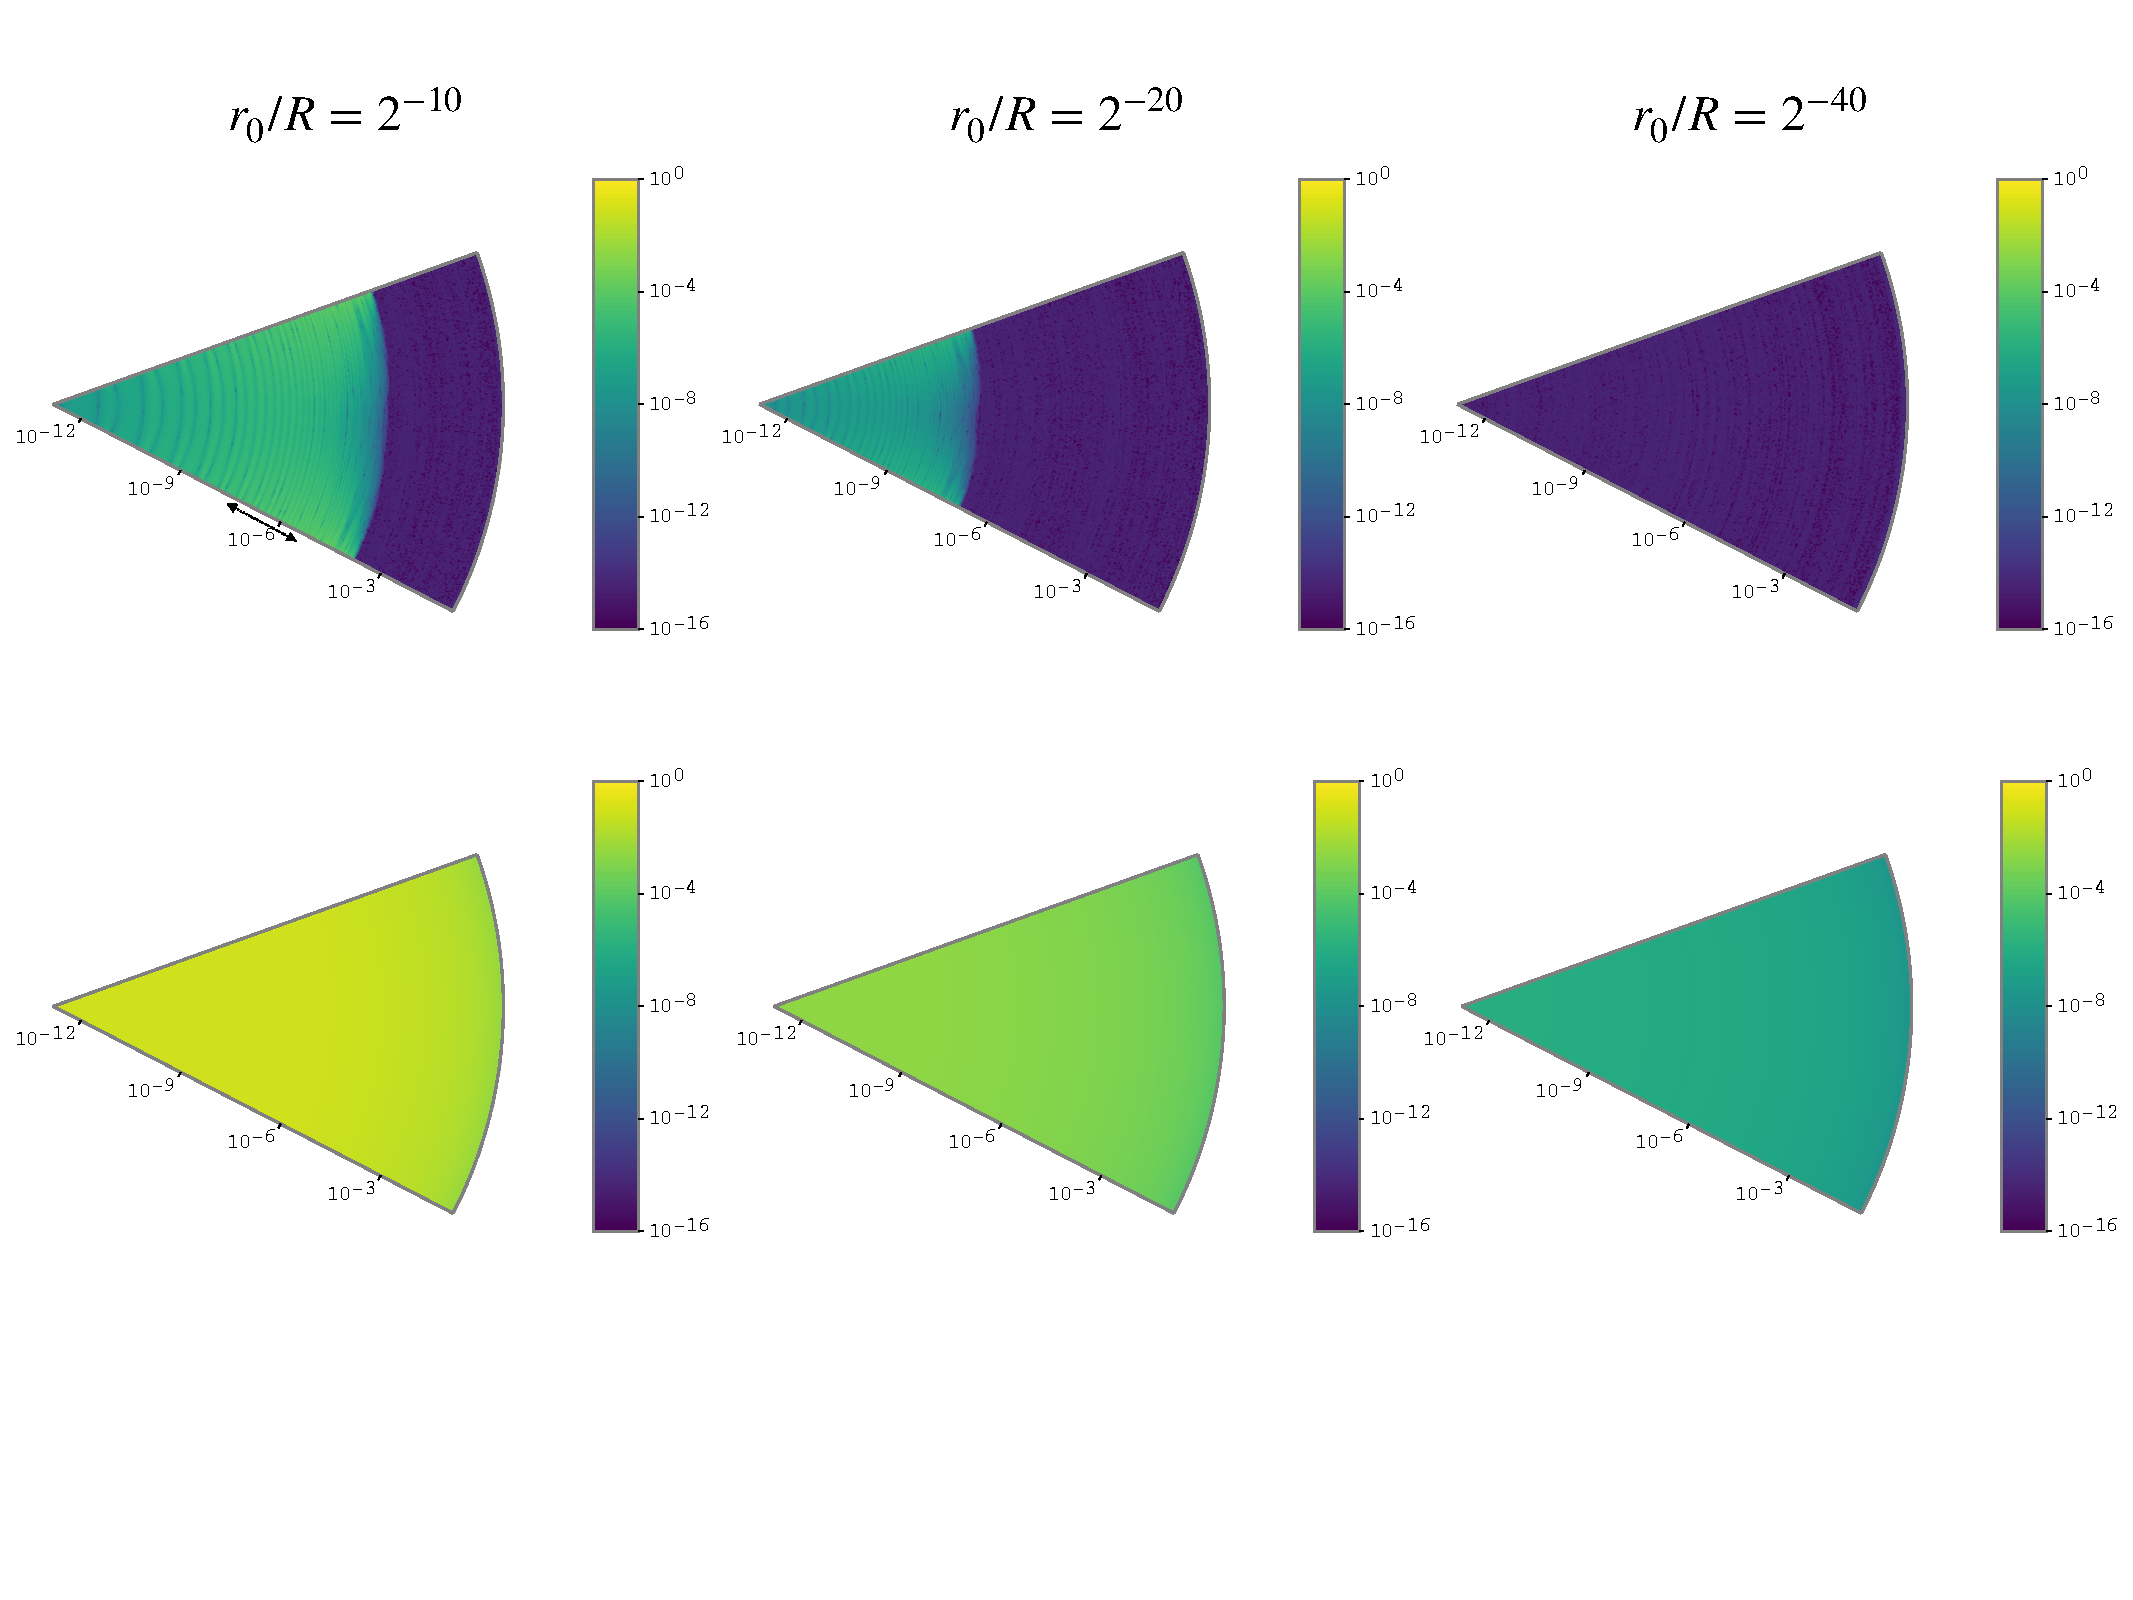
\includegraphics[width=\linewidth]{paper-figs/volume}
\caption{Top row: Solution on the volume after 10, 20, and 40 iterations of re-solve. The solution is computed on a tensor product polar grid, where the evaluation points (targets) are exponentially spaced in the radial direction. The closest target location is approximately $10^{-13}$ away from the corner. Near quadrature is handled via adaptive integration except for the corner panel where the smooth quadrature weights are used. Bottom row: analogous results where the solution is computed using a graded mesh.   }.
\label{fig:vol-plot}
\end{center}
\end{figure}


\subsection{Performance}
In this section, we demonstrate the performance of the solver by solving a scattering problem in the
exterior of a ``broken wheel'' region. The boundary data is given by
\begin{equation}
f(x) = \nabla  \sum_{j=1}^{57} c_{j} \log| \bx - \bx_{j}| \cdot \bnu(\bx) \, , 
\end{equation}
where there is one $\bx_{j}$ located in each of the spokes, one of the $\bx_{j}$ is in the central disc, and the remaining $50$ $\bx_{j}$ are chosen randomly in the exterior of the bounding disc containing the domain. The strengths $c_{j}$ are chosen such that they average to $0$. The domain contains $108$ corners, was discretized using $22240$ nodes and required $105$ iterations to converge to a residue of $10^{-15}$. The matrix at each iteration was applied using an FMM whose tolerance was also set to $10^{-15}$. The solution was computed in $15$ secs, and plotted at a $500\times 500$ grid of targets in $6.5$ secs. All of the results have been computed on a single core on a Macintosh machine with Intel core i5 2.3GHz processors. In~\cref{fig:magnetron}, we plot the scattered field, the boundary data, and the computed density.


\begin{figure}
\begin{center}
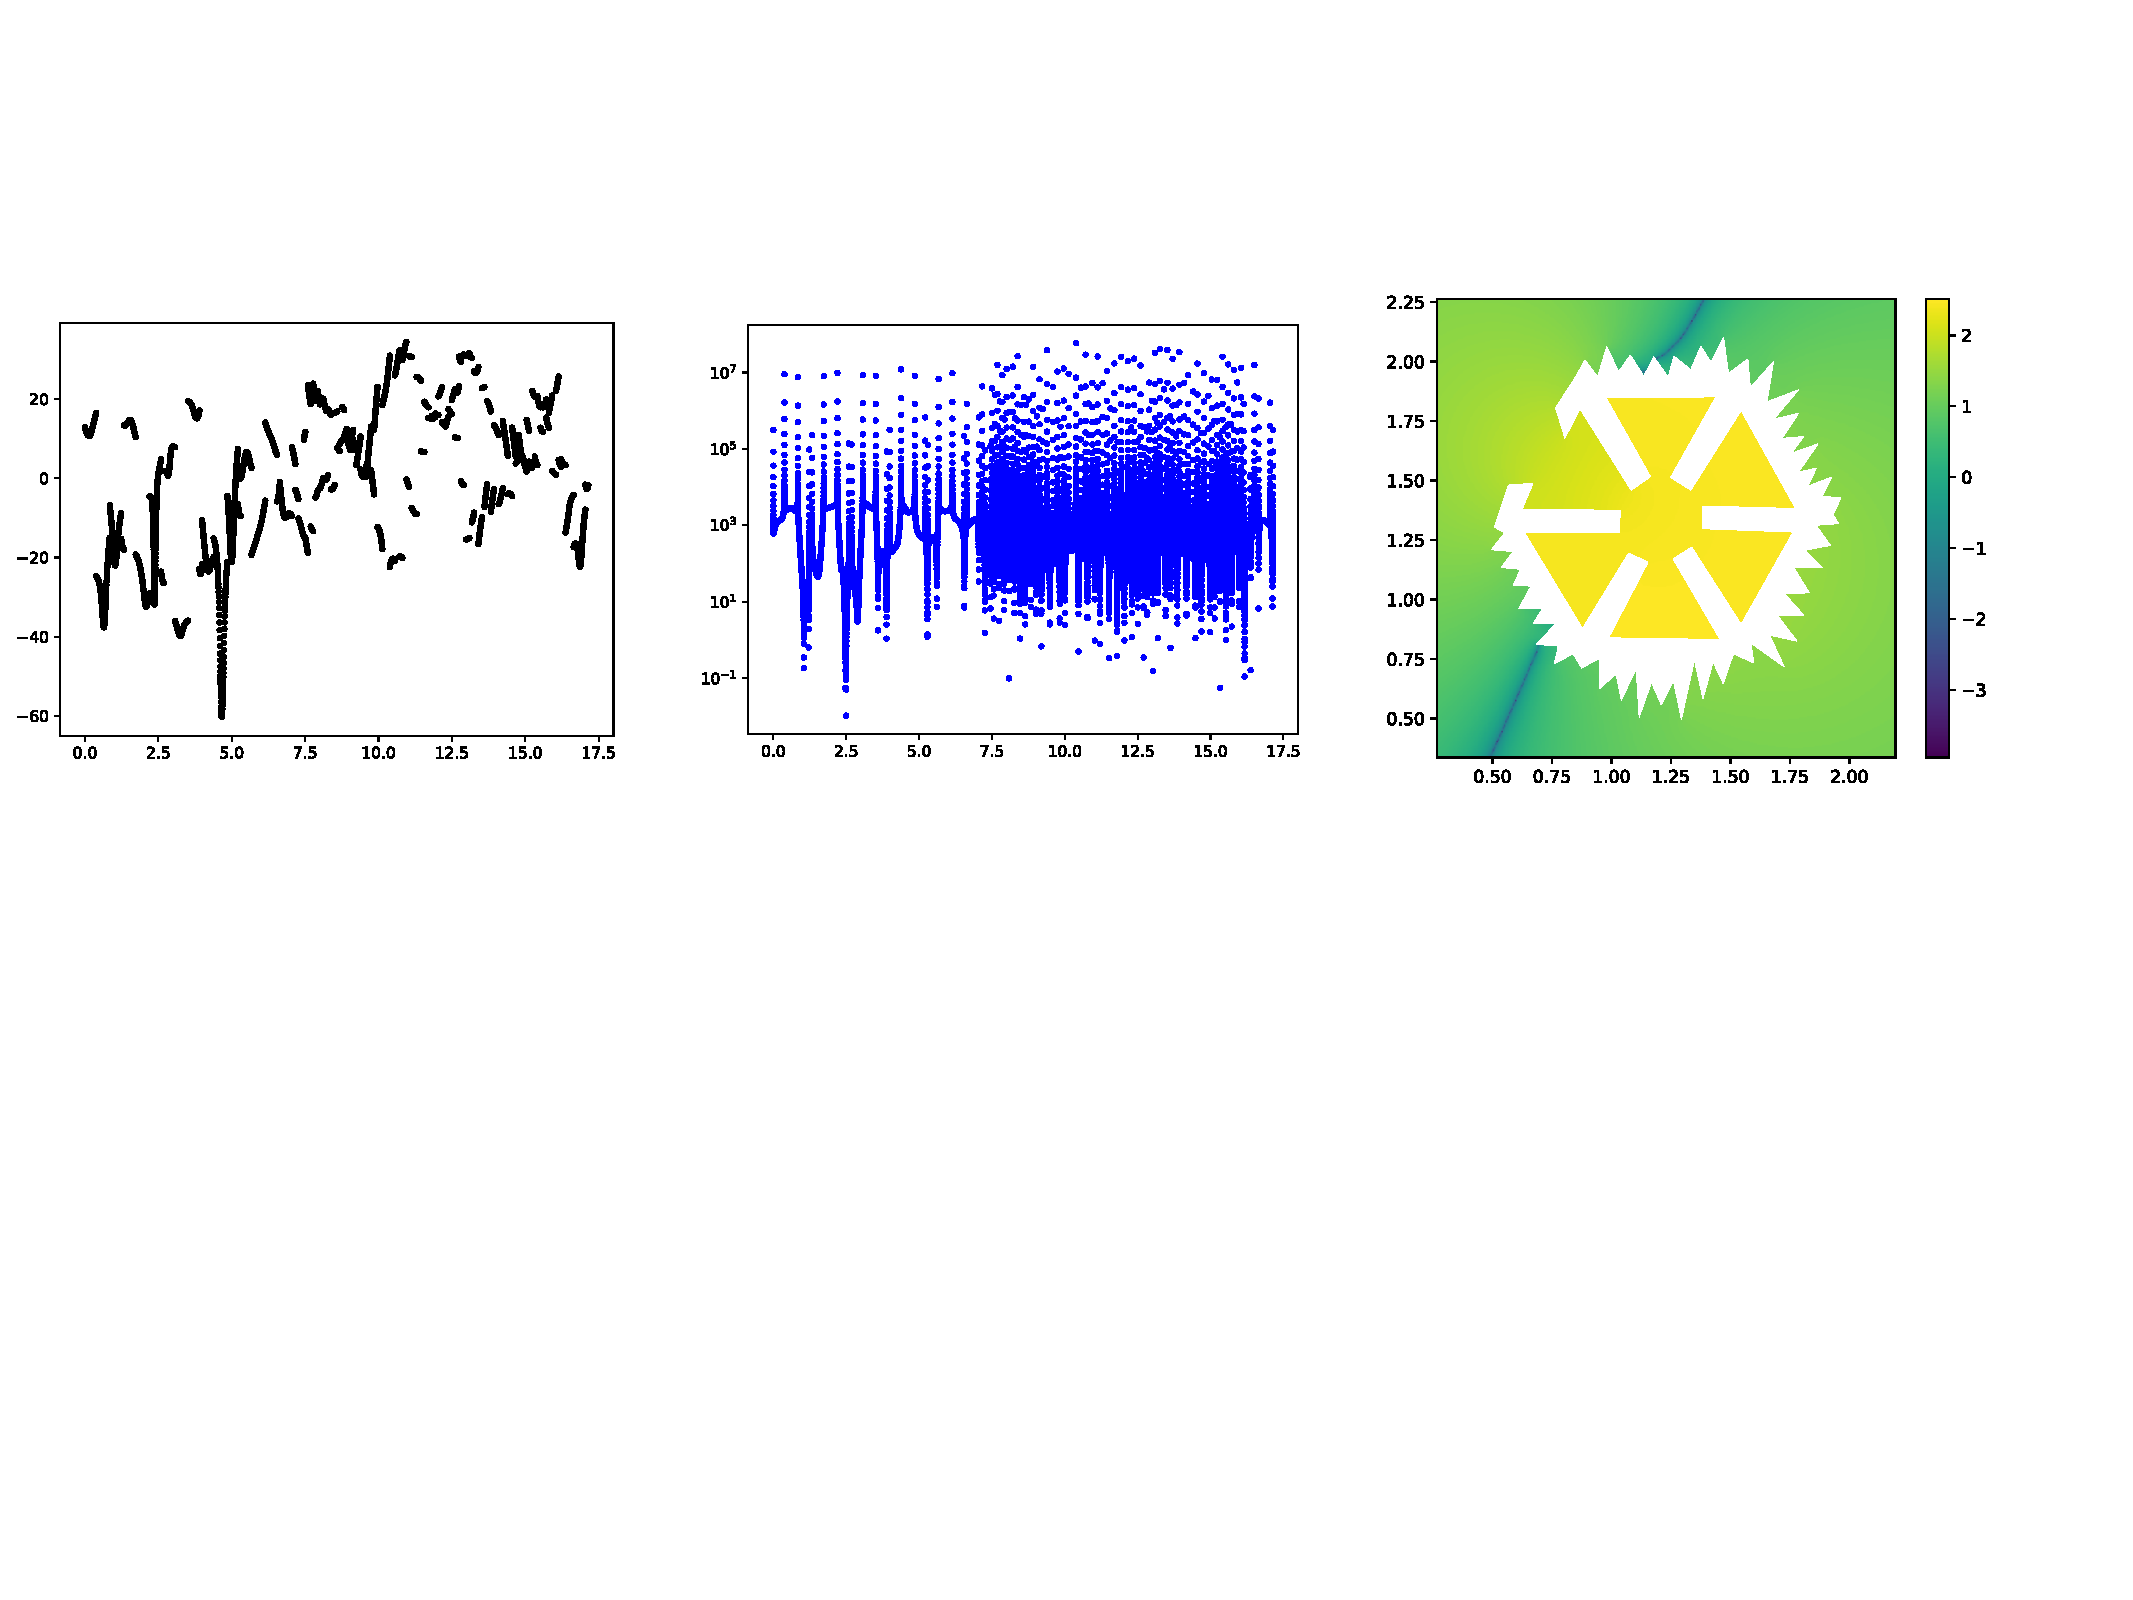
\includegraphics[width=\linewidth]{paper-figs/magnetron}
\caption{(left): Boundary data as a function of arclength, (center): absolute value of density as a function of arclength, and 
(right): $\log_{10}$ of the absolute value of the solution in the volume computed using an FMM.}
\label{fig:magnetron}
\end{center}
\end{figure}
